\documentclass[a4paper, 11pt, oneside]{article} % A4 paper size, default 11pt font size and oneside for equal margins

\usepackage[utf8]{inputenc} % Required for inputting international characters
\usepackage[T1]{fontenc} % Output font encoding for international characters
\usepackage[french]{babel}
\usepackage{csquotes}

\usepackage[twoside, margin=2cm, bindingoffset=0.0cm]{geometry}

\usepackage{hyperref} %For hyperlinks 
\hypersetup{pdfborder=0 0 0}

\usepackage{graphicx}  % Pour images
\graphicspath{{Figures/}}
\usepackage{float}
\usepackage{wrapfig}
\usepackage{xcolor}

\usepackage{tikzit} % Pour les Tikz
\usepackage{tikzscale}
\input{Figures/sample.tikzstyles}
\usetikzlibrary{calc,patterns,angles,quotes}


\usepackage[%backend=biber,
style = ieee,
sorting=none
]{biblatex} %,bibstyle=ieeehttps://www.overleaf.com/project/624dc5f129c1767e8bb8de67
\addbibresource{biblio.bib}
\renewbibmacro*{date}{%
  \iffieldundef{year}
    {\bibstring{nodate}}
    {\printdate}
}

\newcommand{\comment}[1]{}%pour faire des comentaires a plusueures lignes 
\newcommand{\dd}[1]{\mathrm{d}#1}
% TODO trouver une meilleure alternative que ca car ca enleve litalique et apres faire renewcommand \vb*{\}\(
    
\usepackage{physics} %pour \vb*{b}old vectors
%\newcommand{\vb*}[1]{\boldsymbol{#1}}
%\newcommand{\vb*}[][]{}
\begin{document} 
\usetikzlibrary{patterns,patterns.meta}
\tableofcontents
\listoffigures
\listoftables

\newpage
\section*{Introduction}
    % Dire cest quoi leffet cheerios etc \ldots
    %What are cheerios? Is the cheerios effect really an effect or something we created in our reality to rationalise the sogyness of our cereals. Will we be able to eat cereals without making them soggy since we will be so foccused at the cheerios effect. Is the cheerios effect a conspiracy fro cheerios to make us eat soggy cereals or mayb ethey are thirsty and want more time in liquid or maybe they miss their friends inside the bag so the y curve the water to reach them but there was something that they didnt know; the fact that researchers would modelise it and one day two students would choose this effect do simulate it. Maybe that was the objective overall trying to put sense in our worthless lifes. Why would the cheerios be intersted in our lifes? Are we interested in our lifes? Who knows \ldots  
    %Maybe one day we will see what this project meant to but for now we are sailing sailing on the unexpected and in a world filled with possibilities only exploring some possibilities leaving infinite ones untouched. Maybe one day all that will make sense but for now the only thong that makes sense is this paper or maybe not even this so would that mean that our life doesnt have sense/meaning? That is left to the reader maybe it does maybe it doesn't. Maybe it depends how you look at it. It is all filled with maybes however you might look at it as someone scottis and i quote "No you you seee i'm talking facts here i dont do if buts and maybes i do absolutes..." and in that case i have only one thing to say in this paper that should be the case. And with all that said i am leaving you with this paper and a little bit of existentialism, nihilism and our besst wishes about the future.

    Dans le cadre de l'UE Projet en Calcul Scientifique Numérique, nous devions travailler sur un projet, afin de nous apprendre plus en détail, la programmation et le calcul numérique avec un langage compilé, le C. Notre sujet était sur l'"Effet Cheerios", ou l’intéraction d'objets à la surface d'un liquide par l'effet de la gravité et la déformation interfaciale. Cet effet se caractérise par la tension d'une surface liquide sous le poids d'un objet, par exemple une punaise sur l'eau. Lorsque nous ajoutons plusieurs objets sur la même surface, à distance plus ou moins grande, les objets vont potentiellement s'attirer puis créer des tas mobiles. Ce phénomène est notamment visible avec des céréales dans du lait, d'où le nom de Cheerios, célèbre marque de céréales américaine. Pour réaliser à bien ce projet nous avons du faire de nombreuses recherches sur la mécanique des fluides, les collisions inélastiques et nous avons également du faire un travail conséquent sur l'optimisation de notre algorithme.

\section{Le problème et notre modélisation}
    \section{Le problème et notre modélisation}
    % TODO pas sur mais ca peux etre sympa si on se focus plus a cheerios que ceci est pour un cours peut etre ? je sais pas ? qui sais ? pas moi en tot cas. 
    Nous avons tous mangé des céréales ou vu des objets flottant s'attirer ou se repousser entre eux, mais quel est la raison de cette force ? Nous avons essayé de décrire ces interactions dans ce projet.

    Quelque notations : dans ce rapport les vecteurs sont annotés en gras $\vb*{v}$: vecteur $v$
    \begin{table}[H]
        \centering
        \begin{tabular}{ccc}
            \hline
            Nom                & Abréviation & Dimension\\
            \hline
            Rayon de courbure  & $R$         & [$L$]\\
            Surface de tension & $\gamma$    & [$MT^{-2}$]\\ 
            Densité du solide  & $\rho_s$    & [$ML^{-3}$]\\
            Densité du liquide & $\rho_l$    & [$ML^{-3}$]\\
            Densité de l'air   & $\rho_a$    & [$ML^{-3}$]\\
            Nombre de Bond     & $B$         & $1$\\
            \hline
        \end{tabular}
        \caption{Table des variables}
    \end{table}

    \subsection{Effet Cheerios}
    % Ce que Baptiste avait écrit 
    % TODO en parler entre nous pour voir si on fait toute les preuves ou juste decrit le probleme car jai limpression le truc qu on va faire cest tres similaire a celui dans cheerios
        \paragraph*{}{
            Cette partie est plutôt faite pour l'intégrité du rapport. Le lecteur est fortement encouragé à lire "Cheerios Effect"\cite{vella_cheerios_2005} pour avoir une compréhension plus complète du sujet. Les équations viennent principalement de cet article.
        }

        \paragraph*{}{
            Lorsque nous posons un objet sur la surface de l'eau (une aiguille, une punaise ou un cheerio), il est possible que l'objet reste à la surface de l'eau. L'eau va donc se courber, enveloppant une partie de l'objet, sous la masse de celui-ci. Cela se nomme la déformation interfaciale. Elle se retrouve dans la nature avec certains insectes pouvant marcher sur l'eau grâce à cette loi physique. Si nous mettons plusieurs objets de la sorte et qu'ils sont plus ou moins proche, la courbure de l'eau sous ces objets va créer une tension de surface qui attirera les objets jusqu'à qu'ils se touchent. De plus, si nous mettons ces objets dans un récipient, au fil du temps ils vont s'approcher des bords. Nous pouvons également expliquer cela par la tension de surface qui est créée entre le récipient et l'eau qui créera un ménisque.
            }
        % TODO je pense ca serait bien de dire aussi si ils sont le meme signe de courbure ils se raproche si cest lopose ils se repulse.
        \paragraph*{}{
            Nous voulons déterminer comment ces objets réagissent entre eux et les bords d'un récipient et représenter nos résultats de façon numérique et animée. Nous devons, pour cela, calculer tout d'abord les forces intervenant dans ce phénomène.
        } 
        POUR LES PREUVES DES CALCULS LE LECTEUR EST FORTEMENT ENCOURAGE A LIRE LE PAPIER \textit{Cheerios effect}\cite{vella_cheerios_2005} 

        % Ce que Erdi a écrit
        % TODO expliquer de ou viens les forces des angles qui tord la surface ?

        % \begin{figure}[!htb]
        %     \centering
        %     \includegraphics[width=0.5\textwidth]{schema_cheerios_objet_eau.tikz}
        %     \caption{Schéma d'un seul objet proche d'une parois, avec la définition de contact d'angle.}
        %     \label{objet_seul}
        % \end{figure}

        % Expliquer leffet de cheerios.
        
        % TODO peut etre notre propre figure ?
        % \begin{figure}
        %     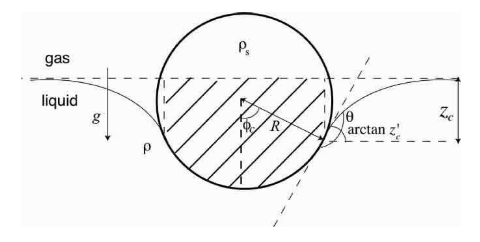
\includegraphics[width = 0.9\textwidth]{boulleflotantedecheerios.png}
        %     \caption{Geometry of a sphere lying at a liquid-gas interface. The shaded area represents the weight of liquid equivalent to the buoyancy force due to hydrostatic pressure acting on the sphere.\cite{vella_cheerios_2005}}
        % \end{figure}
        \begin{figure}[!htb]
            \centering
            \includegraphics[]{schema_geom_sphere_eau.tikz}
            \caption{Géométrie d'une sphère reposant sur une interface liquide-gaz. La partie rayée représente le poids de liquide équivalent à la force de flottabilité du à la pression hydrostatique appuyant sur la sphère. }
            \label{geom_sphere}
        \end{figure}

        Une des raisons pour laquelle les objets flottent est due à la poussée d'Archimède, comme nous pouvons le voir dans la figure \ref{geom_sphere}. Pour que notre sphère reste sur l'interface liquide-gaz elle a besoin que la norme de son poids \(||\vb*{P}||=\frac{4}{3}\pi\rho_{s}gR^3\); doit être équilibrée par la composante de tension superficielle agissant le long de la ligne de contact (circulaire) et par la force de flottabilité due au déplacement du fluide en vrac. La première composante a pour équation :

        \begin{equation}
            2\pi\gamma R\sin{\phi_c}\frac{z_c'}{\sqrt{1+z_c^{'2}}}
            \label{eq:tensionSuperficielle}
        \end{equation}

        Et nous avons également la force de flottabilité par l'équation :
        \begin{equation}
            \pi\rho_l g R^3 \left(\frac{z_c}{R}\sin^2{\phi_c} + \frac{2}{3}-\cos{\phi_c}+\frac{1}{3}\cos^3{\phi_c}\right)
            \label{eq:buoyancyForce}
        \end{equation}

        % TODO expiquer dou ca viens moi ja pas comprie
        % \begin{equation}
        %     2\pi R \phi_c \gamma \sin(\arctan z_c^{'}) = 2\pi\gamma R \sin\phi_c z_c^{'}(1+z_c^{'2})^{-1/2}
        %     \label{eq:wut}
        % \end{equation}

        Nous avons donc l'équilibre des forces donné par :
        \begin{multline}
            \frac{4}{3}\pi\rho_{s}gR^3 =2\pi\gamma R \sin\phi_c \frac{z_c^{'}}{\sqrt{(1+z_c^{'2})}} 
            \\+ \pi\rho_l g R^3 \left(\frac{z_c}{R}\sin^2 \phi_c + \frac{2}{3}-\cos\phi_c+\frac{1}{3}\cos^3 \phi_c\right)
            \label{eq:BalanceOfForces}
        \end{multline}

        % TODO cest quoi $z_c^{'}$??? Un point de contact apparemment 

        Si nous substituons \(\phi_c = \pi - \theta + \arctan z_c^{'}\) et gardons uniquement les termes linéaires en \(z_c^{'}\), nous retrouvons l'expression pour \(z_c^{'}\sin \phi_c\) qui est précis par rapport \textit{à l'ordre linéaire du nombre de Bond}, \(B \equiv R^2/L_c^2\) 

        Nous avons donc:
        \begin{equation}
            z_c^{'}\sin \phi_c = B\left(\frac{2D-1}{3}-\frac{1}{2}\cos \theta + \frac{1}{6} \cos^3 \theta\right) \equiv B\Sigma
            \label{eq:bondsigma}
        \end{equation}
        Avec \(D \equiv \frac{\rho_s}{\rho}\).

        % On peux voir ceci est bien le cas car on observe bien que \(z_c^{'} = 0\) quand \(\theta = \pi/2\) et \(D = 1/2\) cest ce que on satendais car dans ce cas la pousee de archimede seul lui meme est assez pour equilibrer le poids de la sphere sans deformations du liquide.

        L'équation (\ref{eq:bondsigma}) contient deux paramètres sans dimensions; \textit{le nombre de Bond}$B$ et $\Sigma$, qui sont très importants pour notre modélisation.

        Le nombre de Bond vaut:
        \begin{equation}
            B = \frac{(\rho_l-\rho_{a})gR^2}{\gamma} \simeq \frac{R^2}{L_c^2}
        \end{equation}

        Il nous donne la mesure relative de l'importance des effets de gravité et de la tension de surface; si $B$ est tres grand, cela correspond à des particules grandes ou à une tension de surface petite. 

        Pour déterminer $\Sigma$, nous avons besoin de l'angle de contact $\theta$. Pour le trouver nous avons suivi l'article \textit{Lattice Boltzmann Simulation of Capillary Interactions among Colloidal Particles}\cite{lattice_boltzmann_caplilary_interaction} dans le quel ils utilise un angle de contact($\theta$) a satisfier la loi de Young-Dupré supososnt que les particules sont assez petit pour que on puisse negliger les effets de leurs poids sur langle de contact. TODO PAS DU TOUT SUR SI DANS LE NOTRE NOUS AVONS LE DROIT DE FAIRE COMME CA???? (EST QUE ON A UN AUTRE CHOIX ? NOPE :/ DONC ON FAIT TEL QUE CEST NEGLIGABLE DU COUP CEST POUR CA QUE IL NA PAS MARCHE AVEC LES PUNAISES???)
        \begin{equation}
            \cos \theta = \frac{\gamma_{SV}-\gamma_{SL}}{\gamma_{LV}}
        \end{equation}
        Ou $\gamma_{SV,SL,LV}$ est la tension superficielle des interfaces Solide/Vapeur, Solide/Liquide et Liquide/Vapeur.
        et nous n'avons pas pris pour son calcul la masse de l'objet en compte. 
        \begin{equation}
            \theta + \arctan z_c^{'} - \psi_{eq} = \pi 
        \end{equation}
        Avec $\phi_c = \sin^{-1}\left(\frac{\pi}{2}B\right) $ \cite{lattice_boltzmann_caplilary_interaction}. EST QUE CA PREND LA MASSE EN COMPTE OU PAS ?????? LE BOND NUMBER A G ET RHO DONC JE SUPOSSE OUI ???????
        \begin{equation}
            \phi_c = \sin^{-1}\left(\frac{\pi}{2}B\right) = \pi - \theta + \arctan z_c^{'}
            \label{eq:phi}
        \end{equation}
        % Si on combine les equations \ref{eq:bondsigma} et \ref{eq:phi} on a:
        % \begin{equation}
        %     z_c^{'} \sin \left(\sin^-1\left(\frac{\pi}{2}B\right)\right) = B \Sigma
        % \end{equation}
        % \begin{equation}
        %     \Rightarrow z_c^{'}\left(\frac{\pi}{2}B\right) = B \Sigma
        % \end{equation}
        % \begin{equation}
        %     \Rightarrow z_c^{'}\frac{\pi}{2} = \Sigma = \left(\frac{2D-1}{3}-\frac{1}{2}\cos \theta + \frac{1}{6} \cos^3 \theta\right)
        %     \label{eq:zcpi/2=sigma}
        % \end{equation}
        %  Si nous substions \(\phi_c =  \sin^{-1}\left(\frac{\pi}{2}B\right) = \pi - \theta + \arctan z_c^{'} \) On a:
        % \begin{equation}
        %     % \Rightarrow \theta = \pi - \sin^{-1}\left(\frac{\pi}{2}B\right) + \arctan z_c^{'}
        %     z_c^{'} = \tan\left(\sin^{-1}\left(\frac{\pi}{2}B\right)-\pi+\theta\right)
        %     \label{eq:thetafinaly?}
        % \end{equation}
        % Si on remplace le \(z_c^{'}\) dans l'equation \ref{eq:zcpi/2=sigma} avec lequation \ref{eq:thetafinaly} on a:
        % \begin{equation}
        %     \tan\left(\sin^{-1}\left(\frac{\pi}{2}B\right)-\pi+\theta\right)\frac{\pi}{2} =\frac{2D-1}{3}-\frac{1}{2}\cos \theta + \frac{1}{6} \cos^3 \theta 
        % \end{equation}
        % Si on applique deux fois l'egalite trigonometrique: 
        % \begin{equation}
        %     \tan (a+b) = \frac{\tan a + \tan b}{1-(\tan a \tan b)}
        % \end{equation}
        % A TESTER VOIR SI JE ME SUIS PAS TROMPE
        % \begin{equation}
        %     \Rightarrow \frac{\tan \phi_c + \tan (-\pi) + \tan\theta - (\tan \phi_c\tan (-\pi)\tan\theta)}{1-\tan \phi_c \tan(-\pi) - \tan\theta \tan\phi_c - \tan(-\pi)\tan\theta} = \Sigma 
        % \end{equation}
        % \(\tan(-\pi) = 0\)
        % \begin{equation}
        %     \Rightarrow \frac{\tan\phi_c + \tan\theta}{1-\tan\theta\tan\phi_c} = \frac{2D-1}{3}-\frac{1}{2}\cos \theta + \frac{1}{6} \cos^3 \theta
        % \end{equation}
        % Pour le reoudre a la main cest difficile mais numeriquement on peux avoir des solutions. On peux savoir la valeur de $\phi_c$ grace a l'equation \ref{eq:phi} et nous savons que \(D \equiv \frac{\rho_s}{\rho_l}\) alors on peux trouver $\theta$.
        % WUT ???
        % The expression for the slope of the interface in the vicinity of the spherical particle given in (9) is valid for B << 1 (corresponding to a radius of  1mm or smaller for a sphere at an air-water interface) in which case surface tension is very important. The other dimensionless parameter, , can be thought of as a (non-dimensional) resultant weight of the particle once the Archimedes upthrust has been subtracted out. This physical interpretation arises naturally from the vertical force balance condition (8) and (9) since the resultant weight of the object (in the linearised approximation) is simply 

        % L'expression de la pente de l'interface au voisinage de la particule sphérique donnée dans (\ref{eq:bondsigma}) est valable pour B << 1 (correspondant à un rayon de 1mm ou moins pour une sphère à l'interface air-eau), auquel cas la tension superficielle est très importante. L'autre paramètre sans dimension, peut être considéré comme un poids résultant (non dimensionnel) de la particule une fois que la poussée d'Archimède a été soustraite. Cette interprétation physique découle naturellement de la condition d'équilibre de la force verticale (\ref{eq:BalanceOfForces}) et (\ref{eq:bondsigma}) puisque le poids résultant de l'objet (dans l'approximation linéarisée) est simplement 

        %%%%%%%%%%%%%%%%%%%%%%%%%%%%%%%%%%%%%
        % To calculate the interaction energy using the Nicolson approximation, we must also calculate the interfacial displacement caused by an isolated floating sphere, which is determined by the hydrostatic balance \(\gamma\nabla^2h = \rho gh -\) the co-ordinate invariant statement of equation (1). With the assumption of cylindrical symmetry, this becomes:
        TODO EST QUEE CEST POSSIBLE DE METTRE UNE FIGURE ICI DUN TUBE AVEC DE LEAU QUE ON VOIS CEST QUOI H ET X ?
        Nous savons le déplacement interfacial\cite{introfluidcambridge} qui est:
        \begin{equation}
            \gamma \frac{\dd^2h}{\dd x^2} = \rho_l g h
        \end{equation}
        Si nous prenons en compte que l'objet a une symétrie sphérique
        \begin{equation}
            \Rightarrow \frac{1}{r} \frac{\dd}{\dd r} \left( r\frac{\dd h}{\dd r}\right) = \frac{h}{L_c^2}
        \end{equation}
        EN FAITE LASSOCIATIONAU FONCTION BESSEL CA VA MAIS JE SAIS PAS COMMENT PARTIR DE EQUATIONAVEC GAMMA ET DEDUIR UNE SYMETHRIE SPHERIQUE????\\
        Nous pouvons déduire une solution de cette équation avec la fonction de Bessel modifié à l'ordre 0 \cite{introbessel} $(K_0\left(\frac{l}{L_c}\right))$.

        \begin{figure}[H]
            \centering
            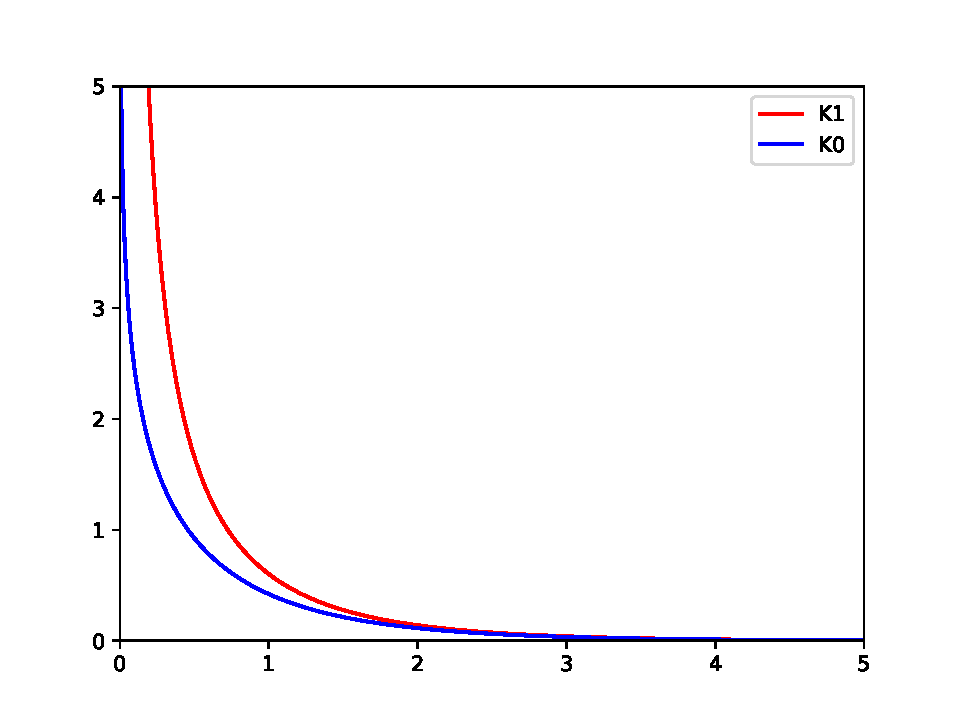
\includegraphics[width = 0.5\textwidth]{Besselk1_K0.pdf}
            \caption{Graphique représentant les fonctions de Bessel modifié à l'ordre 0 et 1}
            \label{fig:bessel}
        \end{figure}
        % TODO faire tel que on aligne a 0 le y et peut etre aller jusq a 6 en x ?
        %%%%%%%%%%%%%%%%%%%%%%%%%%%%%%%%%%%%

        Pour déterminer, maintenant la force d'attraction entre deux objets nous partons du poids effectif d'une sphère sur une interface déformé, que nous donnons comme \(2\pi RB\Sigma\). Nous avons également calculé la déformation interfaciale causée
        par la présence d'une seule sphère. Nous sommes donc capables de calculer l'énergie d'interaction entre deux sphères. Cette énergie est le produit du poids résultant d'une sphère et de son déplacement vertical causé par la présence d'une autre sphère dont le centre est éloigné de l'horizontale d'une distance horizontale $l$. Nous pouvons donc écrire l'énergie, $E(l)$, comme suit :
        \begin{equation}
            E(l)=-2\pi\gamma R^2b^2\Sigma^2K_0\left(\frac{l}{L_c}\right)
            \label{eq:energyInteraction}
        \end{equation}
        Avec $L_c$ la longueur capillaire.

        Nous pouvons donc trouver la force d'interaction $F(l)=-\frac{dE}{dl}$, ce qui donne :
        \begin{equation}
            \boxed{
                F(l)=-2\pi\gamma RB^{5/2}\Sigma^2K_1\left(\frac{l}{l_c}\right)
            }
            \label{eq:ForceInteraction}
        \end{equation}

        Nous voyons ( voire ) ?????? bien grace a la figure \ref{fig:bessel} que des que $l/L_c>5$ notre force va etre tres faible et inversement quand $l/L_c << 1 $ la force de atraction va etre tres eleve. La force entre objets flottants depens de la distance entre eux exponentielement. A REPHRASER CE PARAGRAPH 

        
        

        % TODO dans le code ajouter un buoyancy force qui calcule la ousee de archimede et dis si notre objet flotte ou pas si il flotte pas on peux metre un option tel quel il prend la valeur automatique ??? Ou on le neglige ????
        % TODO On mets les formules et peut etre demontrer ou ils viennent et surtout les cas ou on peux utiliser ces formules les cas ou ca marche pas etc\ldots
        % TODO SCHEMA deux cheeios et sur le schema on monre l Rayon de courbure etc...

        % TODO peut etre rephrase, lidee est la mais lexecution nest pas   
        %\newpage
        \subsection{Force des bords}
            \begin{wrapfigure}{r}{0.25\textwidth}
            \centering
                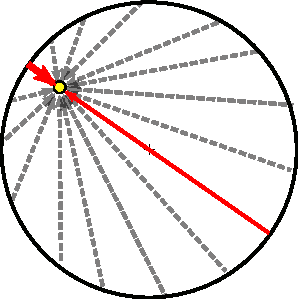
\includegraphics[width = 0.2\textwidth]{Figure_Force_Bord.pdf}
                \caption{Schéma des forces des bords.}
                \label{fig:Force_Bord_schéma}
            \end{wrapfigure}
            TODO JAI AJOUTE DES CHOSES ICI MAIS PEUT ETRE REPHRASHER
            Maintenant que nous avons vu l'application des forces entre objets, nous allons expliquer les forces entre les bords et les objets. La force se calcule de la même manière qu'entre deux objets (equation \ref{eq:ForceInteraction}) car la force depend du rayon de courbure($R$), nomre de Bond($B$), Sigma($\Sigma$), longueur capillaire($L_c$) et de la distance entre deux points($l$) de force et tout ces parametres peuvent etre trouver pour le bord. Pour la force appliquée par les bords sur les objets nous avons, à la place de calculer les forces à chaque point du cercle, opté d'utiliser la symétrie dun cercle. Nous avons remarqué que la plupart des forces s'annulent entre elles (en gris) et il nous reste seulement deux forces (en rouge) qui interagissent comme le montre la figure\ref{fig:Force_Bord_schéma}. Les seuls paramètres à changer sont le nombre de Bond et l'angle de contact, que nous prenons à 45 degré, angle du ménisque formé par l'eau dans un récipient en verre. 
            % Pour la force appliquée par les bords sur les objets nous avons décidé de ne pas calculer les forces de chaque point du bord, au lieu de cela nous avons utilisé la symétrie d'un cercle (nos bords étant un cercle). Seulement deux forces de bords vont s'appliquer sur un objet, les autres s'annulant par symétrie, comme le montre la figure \ref{fig:Force_Bord_schéma}
            % \begin{figure}[H]%[!htb]
            %     \centering
            %     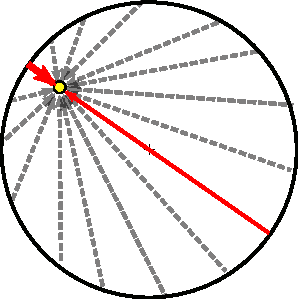
\includegraphics{Figure_Force_Bord.pdf}
            %     \caption{Schéma des forces des bords.}
            %     \label{fig:Force_Bord_schéma}
            % \end{figure}

\section{Méthodes numériques et algorithme}
    \subsection{Integration de Verlet}
        Pour déterminer nos coordonnées, vitesses et accélérations en fonction du temps nous avons opté pour l'intégration de Verlet. L'intégration de Verlet est un algorithme simple à mettre en place et qui permet de conserver l'énergie dans le système. L'algorithme utilise le développement limité de Taylor de notre vecteur position à l'ordre 3.

        %On prouve lintegration de verlet et montre que on peux lutiliser pour notre probleme
        %Si on applique le developement limite de x on peux deduir les positions suivant
        Démonstration du développement limité de Taylor Young de $f(x)$ au point $x_0$\cite{agarwal_introduction_2011} :% TODO citer le livre de introduction a lanalyse complexe et numerique dans la mir 
        \begin{equation}
            \mathrm{DL}_n f(x) = \sum_{i=0}^{n}\frac{f^{(i)}(x_0)}{i!}(x-x_0)^i+ o((x-x_0)^n)
        \end{equation}
        Si on applique le développement limité d'ordre 3 à la position($\vb*{x}(t+\dd t)$) au point $t+\dd t$ on a l'équation suivante avec $t_0$ comme le pas de temps précédent :
        % On a ca avec le developement limilte a $t$ et $t_0$ cest le pas temps precedent
        \begin{equation}
            \Rightarrow\mathrm{DL}_3 \vb*{x}(t) = \vb*{x}(t_0)+\vb*{x}^{'}(t_0)(t-t_0)+\frac{\vb*{x}^{''}(t_0)}{2!}(t-t_0)^2 +o((t-t_0)^3)
        \end{equation}
        Si $t_0$ est le pas de temps précédent, $\vb*{x}^{'}(t)$ vitesse et $\vb*{x}^{''}(t)$ l'accélération, nous avons :
        \begin{equation}
            \Rightarrow\mathrm{DL}_3 \vb*{x}(t+\dd t) = \vb*{x}(t)+\vb*{x}^{'}(t)(t+\dd t-t)+\frac{\vb*{x}^{''}(t)}{2!}(t+\dd t-t)^2+o(t+\dd t-t)
        \end{equation}
        \begin{equation}
            \Rightarrow \mathrm{DL}_3 \vb*{x}(t+\dd t)= \vb*{x}(t)+\vb*{v}(t)(\dd t)+\frac{\vb*{a}(t)}{2!}(\dd t)^2+o(\dd t^3)
        \end{equation}
        L'erreur sur le temps $t_n$ est de l'ordre de $o(\exp(Lt_n)\dd t^2)$ % TODO pas sur de ici

        Notre accélération ne dépendant pas du changement de vitesse mais de l'équation (\ref{eq:ForceInteraction}), nous pouvons calculer l'accélération à partir du principe fondamental de la dynamique avec une masse constante. Il est important de faire cela après le calcul de position mais avant la vitesse car la position prend l'accélération précédente et la vitesse prend celui de avant et pendant le temps.
        \begin{equation}
            \label{PFD}
            \sum  \vb*{F} = m\vb*{a} \Longrightarrow \vb*{a} = \frac{\sum \vb*{F}}{m}
        \end{equation}

        Maintenant nous avons la nouvelle position et l'accélération, nous pouvons calculer la nouvelle vitesse de la même façon en utilisant le développement limité de Taylor Young à l'ordre 2 car après l'accélération nous ne connaissons pas le \textit{jerk} (changement de l'accélération par rapport au temps).
        \begin{equation}
            \mathrm{DL}_2\vb*{v}(t) = \vb*{v}(t_0) + \vb*{v}^{'}(t_0)(t-t_0) + o((t-t_0)^2)
        \end{equation}
        %Si $t_0$ cest le pas de temps precedent ($t_0 = $) et $\vb'{v}(t)$ l'acceleration, nous avons:
        De la meme façon que on a fait notre position ($\vb*{x}(t+dt)$) nous pouvons l'appliquer a la vitesse aussi, nous avons:
        \begin{equation}
            \mathrm{DL}_2\vb*{v}(t+\dd t) = \vb*{v}(t) + \vb*{a}(t)(\dd t) + o(\dd t^2)
        \end{equation}

        % TODO jai limpression que la formule de bas viens de qqpart mais je sais pas de ou ? peut etre une meilleur approwximation ???????
        Comme nous connaissons l'accélération au pas de temps suivant et precedent en meme temps on peux avoir une meilleur approximation de notre vitesse en utilisant le théorème des accroissements fini. TODO ICI JE SUIS PAS DU TOUT SUR ????
        \begin{equation}
            \label{eq:verletVitesse}
            \vb*{v}(t+\dd t) = \vb*{v}(t)+\frac{\vb*{a}(t)+\vb*{a}(t+\dd t)}{2}\dd t 
        \end{equation}
        % est que on mets ca sur lanexe ?
        % (voir lanexe pour le developement du calcul) 
        %        \[DL_3 x(t+\dd t)= x(t)+x^{'}(t)(\dd t)+\frac{x^{''}(t)}{2!}(\dd t)^2\]
        %= & x(t)+x^{'}(t)(t+\dd t-t)+\frac{x^{''}(t)}{2!}(t+\dd t-t)^2\\
        %Essai avec $x(t)$\[DL x(t) = x(t_0)+x^{'}(t_0)(t-t_0)+\frac{x^{''}(t_0)(t-t_0)^2}{2!}\]
    \subsection{Collisions}
        \subsubsection{Collisions Objet-Objet}
            %Ce que Baptiste a fait 
            Pour les collisions, nous sommes partis sur un modèle assez simple qui itère chaque objet et regarde si la distance entre leurs centres est plus petite que leurs rayons additionnés. Si c'est le cas, nous disons qu'il y a collision entre eux et nous appliquons la collision avec la conservation du momentum. 
            % TODO peut etre metre une partie de cela dans la subsection conclusions ? 
            Nous avons mis en place les collisions entre deux objets mais également entre un objet et les bords. Le fonctionnement des collisions entre ces deux cas est très différent. Pour les collisions entre objets, nous prenons dans un premier temps le vecteur normé de collision, dans le sens de objet 1(A) vers objet 2(B):
            % TODO peut etre preciser que cest pour le calcul de A et pour B il faux le refaire ? ou pas jsp ???
            \begin{equation}
                \vb*{c} = \frac{\vb*{AB}}{||\vb*{AB}||} \longrightarrow ||\vb*{c}|| = 1
            \end{equation}
            Puis nous calculons la vitesse relative $\vb*{v}_{rel} = \vb*{v}_A - \vb*{v}_B$ pour comprendre comment les 2 objets vont s'affecter. Après cela, nous trouvons la vitesse des objets lors de la collision afin de nous être utile pour déterminer l'impulsion qui suivra la collision :
            % TODO peut etre preciser que la vitesse de collision nest pas un vecteur ?
            \begin{equation}
                v_{col}=\vb*{v_{rel}}\cdot\vb*{c}
            \end{equation}
            Nous ajoutons à cette vitesse un coefficient compris entre 0.2 et 0.7 car nous n'avons pas de collisions élastiques parfaites. Il faut cependant faire attention à cette constante; Si elle est trop basse, les objets n'auront pas le rebond nécessaire et vont commencer à s'entrer dedans. Si elle est trop haute, les objets vont, à l'inverse, beaucoup rebondir. Toutefois, plus notre pas de temps est petit, plus ces effets vont disparaître.
            
            % TODO pas sur de ici faut tester (note pour moi dans le futur)
            Le signe de la vitesse de collision nous donne si les objets viens vers eux($v_{col} > 0$) ou se elloigne($v_{col} < 0$) car cest possible que quand on a fait la collision pour un objet que on a bien modifie lautre objet aussi donc parfoit on a besoin de faire ca une seule foir et parfois entre temps en faisant tout les collisions il peux revenir. % La phrase na pas de sens jsp ???
            
            % TODO peut etre faire un schema pour montrer les vecteurs que on parle ?
            Si la vitesse de collision est plus grande que 0; on fais la conservation de momentum.
            
            Impulse ($I$)
            \begin{equation}
                I = \frac{2v_{col}}{m_A + m_B}
            \end{equation}
            \begin{equation}
                \vb*{v}_A^{'} = \vb*{v}_A - Im_B\vb*{c}
            \end{equation}
            \begin{equation}
                \vb*{v}_B^{'} = \vb*{v}_B + Im_A\vb*{c}
            \end{equation}
            %Ce que Erdi a fait
            % Expliquer comment on a deduit que les collisions etait des collisions inelastic parfait et metre les equations utilise
            % Pour les collisions, nous sommes partis sur un modèle assez simple qui itère chaque objet et regarde si la distance entre eux est plus petite que leur rayons additionnés on dis que il ya une collision et on applique les collisions et la conservation de momentum.
            

        \newpage
        \subsubsection{Collision des bords}
            \begin{wrapfigure}{r}{0.25\textwidth}
                \centering
                \includegraphics[width = 0.15\textwidth]{rebond.tikz}
                \caption{Schéma d'un rebond d'un objet sur un bord}
            \end{wrapfigure}
            Et aussi on fait des collisions de bord aussi.
            Pour les collisions de bord on a fait tel que si notre objet dépassait le bord de tres peut on inverse le vecteur vitesse par rapport a la normale. Et apres multiplie ce vecteur par un coefficient de collision ($C_c$), $0 \leq C_c \leq 1$ qui simule l'absorbions de l'énergie a chaque collisions. 
            % TODO la fiqure ici cest broullion objective de montrer la norme tangent et la vitesse
            \begin{equation}
                \vb*{v}^{'} = (\vb*{v}\cdot\vb*{n})\vb*{n} +(\vb*{v}\cdot\vb*{t})\vb*{t}
            \end{equation}
            On inverse le coefficent de la normale pour le faire `rebondir'
            \begin{equation}
                \Rightarrow\vb*{v}^{'} = -(\vb*{v}\cdot\vb*{n})\vb*{n} + (\vb*{v}\cdot\vb*{t})\vb*{t}
            \end{equation}
            
            % TODO ca fait qqchose cheloue dans le rendu mais en socuprait de ca a la fin?
\section{Comment on a concue notre probleme}
    \begin{itemize}
        \item On a pris l'interaction des forces totale sur chaque particule par la fonction dans l'article `Cheerios effect'
        \item et de ca on deduis la force que reagis a chaque cheerios pour un pas de temps 
        \item Check si il ya des collisions ou pas et si il ya on change les proprietes des cheerios par rapport aux collisions
        \item De la force en utilisant l'integration de verlet et le principe fondamentale de la dynamique somme forces = derive (masse*vitesse) on peux changer les positions des cheerios
    \end{itemize}
    % Je panse pas que on a besoin de inclure ca car si on fait bien notre taff dans le rapport ils devrait le comprendre et dans le code le code cest comme si cetait ecris en psuedo code 
    % Psuedocode:
    % Prends les donnees 
    % Pour tout les pas de temps(NT)
    %     Parcour chaque objets et compare entre eux si il ya collision.
    %         Si oui 
    %             Applique collisions comme TODO si on va utiliser ca citer lequation dans le quel on en parle
    %         si non
    %             applique force 
    %     pour chaque objet applique force du bord
    %     pour chaque objet integration de verlet
    %     ecriture dans le fichier donnees 
    
\section{Les choses a ameliorer}
    \begin{itemize}
        \item Code en $O(NT\,n^2)$ et peux etre ameliorer enn$O(NT\, n\log n)$ en faisant le calcul de collisions plus inteligament a la place de une recherche exasthive et en calculant une seule fois le \textit{millieu} des forces de chaque particule pour avoir un centre de atraction et comme ca on calcule le centre de attraction regarde si on a des collisions ou pas et a la fin ajoute les forces du bords a chaque particule
        \item pour linstant on utilise les equations \textit{aproximatives} on peux les essayer de les resoudres sans approximations en utilisant laproximation de Nicholson(fine difference method)
        \item le code marche seulement pour les objets ronds faux ajouter une facon plus complexe pour plus de objets
    \end{itemize}
\section*{Conclusion}

\newpage
\thispagestyle{empty}
\nocite{*}
\addcontentsline{toc}{section}{Bibliographie}
\printbibliography[title = Bibliographie]

\end{document}